% based on a template made by the university of cologne
% http://www.mi.uni-koeln.de/wp-MIEDV/wp-content/uploads/2016/07/LaTeX-Vorlage.zip - 2023-11-02
\documentclass[12pt,a4paper]{scrartcl}

\addtokomafont{sectioning}{\rmfamily}
%\usepackage[ngerman]{babel}% deutsches Sprachpaket wird geladen
\usepackage[T1]{fontenc} % westeuropäische Codierung wird verlangt
\usepackage[utf8]{inputenc}% Umlaute werden erlaubt
\usepackage[usenames]{color} % Erlaubt die Benutzung der namen im Farbpaket und deren Änderung
\usepackage{amsmath} % Erweiterung für den Mathe-Satz
\usepackage{amssymb} % alle Zeichen aus msam und msmb werden dargestellt
\usepackage{graphicx} % Graphiken und Bilder können eingebunden werden
%\usepackage{multirow} % erlaubt in einer Spalte einer Tabelle die Felder in mehreren Zeilen zusammenzufassen
\usepackage{enumerate} % erlaubt Nummerierungen
\usepackage{url} % Dient zur Auszeichnung von URLs; setzt die Adresse in Schreibmaschinenschrift.
\usepackage[center]{caption}  % Bildunterschrift wird zentriert
%\usepackage{subfigure} % mehrere Bilder können in einer fugure-Umgebung verwendet werden
%\usepackage{longtable} % Diese Umgebung ist ähnlich definiert wie die tabular-Umgebung, erlaubt jedoch mehrseitige Tabellen.
%\usepackage{paralist} % Modifikation der bereits bestehenden Listenumgebungen
\usepackage{lmodern}% Für die Schrift
\usepackage[hidelinks]{hyperref} % Links und Verweise werden innerhalb von PDF Dokumenten erzeugt
%\usepackage{wrapfig} % Das Paket ermöglicht es von Schrift umflossene Bilder und Tabellen einzufügen.
\usepackage{latexsym} % LaTeX-Symbole werden geladen
\usepackage{tikz} % Erlaubt es mit tikz zu zeichnen
\usepackage{tabularx} % Erlaubt Tabellen
\usepackage{algorithm} % Erlaubt Pseudocode
\usepackage{color} % Farbpaket wird geladen
%\usepackage{stmaryrd} % St Mary Road Symbole werden geladen
\usepackage{physics}

\numberwithin{equation}{section} % Nummerierungen der Gleichungen, die durch equation erstellt werden, sind gebunden an die section
\newcommand{\HRule}{\rule{\linewidth}{0.7mm}}
\newcommand{\pu}[1]{\ensuremath{\mathrm{#1}}}

% disable commands
\renewcommand{\[}{} % math block start
\renewcommand{\]}{\noindent} % math block end
\newcommand{\tightlist}{} % created in enumerations

\hypersetup{
  pdftitle={B 3.3},
  pdfcreator={LaTeX via pandoc}}

\setcounter{secnumdepth}{6}
\setcounter{tocdepth}{6}

\begin{document}
\begin{titlepage}
	\pagestyle{empty}

	\begin{center}

	\textsc{\LARGE Universität zu Köln }\\ [0.4cm]
	\textsc{Mathematisch-Naturwissenschaftliche Fakultät} \\[1.5cm]

	\includegraphics[width=0.45\textwidth]{uni}\\[1.5cm]  % Uni-Logo wird geladen

	\textsc{\Large Praktikum~B}\\[2mm]
	\textsc{}\\[10mm]
	\HRule \\[0.4cm]

		{	\Huge \bfseries B 3.3}\\[0.4cm]
			{	\huge \bfseries Reichweite von \(\alpha\)-Strahlen}\\[0.3cm]
	
	\HRule \\[3cm]

			\textsc{\Large Catherine Tran } \\[3pt]
		\textsc{\Large Carlo Kleefisch } \\[3pt]
		\textsc{\Large Oliver Filla } \\[3pt]
		
% 	\begin{center}
% 	\textsc{\Large Catherine~Tran } \\[3pt]
% 	\textsc{\Large Carlo~Kleefisch } \\[3pt]
% 	\textsc{\Large Oliver~Filla } \\[3pt]
% 	\end{center}
	\end{center}
\end{titlepage}

\newpage
\tableofcontents
\newpage

\hypertarget{einleitung}{%
\section{Einleitung}\label{einleitung}}

In diesem Versuch wird die Wechselwirkung von \(\alpha\)-Teilchen mit
den Elektronen der Atomhülle und der damit verbundene Abbremsung durch
inelastische Stöße untersucht. Des Weiteren werden das Phänomen des
\(\alpha\)-Zerfalls, Bremsvermögen, Reichweite in Luft und Folie sowie
Energie-Straggling durch die Aufnahme von \(\alpha\)-Spektren mithilfe
eines Sperrschichtdetektors studiert.

\hypertarget{theoretische-grundlagen}{%
\section{Theoretische Grundlagen}\label{theoretische-grundlagen}}

\hypertarget{bethe-bloch-gleichung}{%
\subsection{Bethe-Bloch-Gleichung}\label{bethe-bloch-gleichung}}

Bewegte und geladene Teilchen werden durch Interaktion mit Materie
abgebremst, indem sie durch Stöße mit Atomkernen sowie Elektronen
wechselwirken. Schwere Teilchen mit einer Ruhemasse \(M_0\gg m_e\)
deutlich größer der Elektronen-Ruhemasse \(m_e\) werden primär durch die
Wechselwirkung mit Atomkernen gebremst, wodurch die Atome angeregt und
ionisiert werden können.

Die Bethe-Bloch-Gleichung beschreibt den Verlust von Energie \(E\) pro
Strecke \(x\) durch das Durchfliegen eines homogenen Bremsmediums.

Dazu werden die Dichte \(\rho\), die Atommassenzahl \(A\) und die
Ladungszahl \(Z\) des Bremsmediums benötigt. Dabei wird von einem
homogenen Medium mit \(N\) Atomen pro Kubikzentimeter und der
Kernladungszahl \(Z\cdot e\) ausgegangen, wobei \(e\) die
Elementarladung darstellt. \(\beta\) ist der Quotient aus
Geschwindigkeit \(v\) und Lichtgeschwindigkeit \(c\), der auch in der
Relativitätstheorie verwendet wird.

\[
\begin{eqnarray}
    N &=& \frac{\rho\cdot N_A}{A} \\
    \beta &=& \frac{v}{c}
\end{eqnarray}
\]

Ebenso werden die Ladungzahl \(z\) und Geschwindigkeit \(v\) des
Projektils sowie die Elektronen-Ruhemasse \(m_e\) verwendet. Weiterhin
sind das mittlere Ionisationspotential \(\bar I\), gemittelt über alle
Atomschalen des Bremsmediums, sowie eine Korrektur \(c_K\) notwendig.
Letztere beschreibt den fehlenden Beitrag der \(K\)-Schalen-Elektronen
bei kleinen Geschossenergien.

\[
\begin{eqnarray}
    -\frac{\mathrm dE}{\mathrm dx} &=&
        \frac{4\pi z^2 e^4}{m_e v^2} NZ
        \left[
            \ln\left(\frac{2mv^2}{\bar I}\right)
            - \ln\left(1 - \beta^2\right)
            - \beta^2
            - \frac{c_K}{Z}
        \right]
        \label{BetheBloch}
\end{eqnarray}
\]

\hypertarget{herleitung}{%
\subsubsection{Herleitung}\label{herleitung}}

Im Folgenden werde die Bethe-Bloch-Gleichung für schwere, schnelle und
geladene Projektile wie \(\alpha\)-Teilchen hergeleitet.

Hierbei wird eine quasi-klassische Betrachtung des Stoßvorganges
angenommen. Da das Projektil sehr schwer im Vergleich zu Elektronen ist,
kann seine Bewegung als näherungsweise linear angenommen werden.
Weiterhin wird das Elektron als schwach gebunden und ruhend angenommen.
Diese Annahmen können durch die hohe Geschwindigkeit und Masse des
Projektils getätigt werden.

Da das Projektil das Elektron passiert, heben sich sämtliche
Wechselwirkungen parallel zur Flugbahn auf. Dadurch muss nur die
orthogonale Komponente der Coulomb-Kraft \(\vec F\) betrachtet werden,
die durch die Ladungen des Projektils \(Q=ze\) und des Elektrons
\(q=-e\) im Abstand \(\vec r\) erzeugt wird. Der Betrag des Abstands
kann durch die Wegstrecke \(x\) des Projektils sowie den orthogonalen
Abstand \(b\) der Flugbahn und des Elektrons als \(r^2=x^2+b^2\)
beschrieben werden.

\[
\begin{eqnarray}
    \vec F &=& \frac{Qq}{r^2} \frac{\vec{r}}{\left|\vec r\right|} \\
    \vec F &=& -\frac{ze^2}{x^2+b^2} \frac{\vec{r}}{\left|\vec r\right|}
\end{eqnarray}
\]

Weiterhin kann die Kraft durch das elektrische Feld \(\vec E\) des
Projektils und die Ladung des Elektrons \(q=-e\) beschrieben werden
\(\eqref{F=E}\). Diese Gleichung wird integriert, um den Betrag des
Impulsübertrages \(\left|\Delta p_e\right|\) zu ermitteln. Dabei wird
die Integration nach der Zeit durch eine Integration nach dem Ort
substituiert, was durch die konstante Geschwindigkeit \(v\) ermöglicht
wird. Weiterhin wird die Symmetrie ausgenutzt, wodurch nur noch über die
orthogonale Komponente integriert werden muss.

\[
\begin{eqnarray}
    \vec F &=& -e \vec E \label{F=E} \\
    \left|\Delta p_e\right| &=& \int \vec F \mathrm dt \\
    \left|\Delta p_e\right| &=& \frac{e}{v} \int E_\perp \mathrm dx
\end{eqnarray}
\]

Darauf wird der Gauß'sche Integralsatz angewendet. Weiterhin wird der
Energieübertrag \(\Delta E\) durch die kinetische Energie
\(E=\frac{p^2}{2m_e}\) des Elektrons dargestellt. Dann kann über einen
hohlen Zylinder vom Radius \(b_\mathrm{min}\) bis \(b_\mathrm{max}\)
integriert werden. Sinnvolle Integrationsgrenzen sind notwendig, da das
Integral sowohl bei \(x=0\) als auch bei \(x=\infty\) divergieren würde.

\[
\begin{eqnarray}
    -\left(\frac{\mathrm dE}{\mathrm dx}\right)
        &=& \frac{4\pi z^2 e^4}{m_ev^2}
            \ln\left[\frac{b_\mathrm{max}}{b_\mathrm{min}}\right]
            \propto \frac{z^2}{v^2}
\end{eqnarray}
\]

Nun werden relativistische Korrekturen durchgeführt, die zu der
vollständigen Bethe-Bloch-Gleichung \(\eqref{BetheBloch}\) führen.

\hypertarget{diskussion-des-kurvenverlaufs}{%
\subsubsection{Diskussion des
Kurvenverlaufs}\label{diskussion-des-kurvenverlaufs}}

Bei niedrigen Energien steigt die Kurve beinahe linear an. Dies ist
darauf zurückzuführen, dass ein langsames \(\alpha\)-Teilchen aufgrund
der langen Wirkzeit beim Durchqueren des Mediums zufällig Elektronen
aufnimmt und abgibt. Dies wiederum reduziert die die effektive Ladung
des \(\alpha\)-Teilchens und somit den Energieverlust.

Für \(\alpha\)-Teilchen findet sich bei kinetischen Energien von etwa
\(0.5-0.6\mathrm{\,MeV}\) ein Peak. Bei der Verbreiterung des Peaks der
Verteilung sind nicht-statistische Effekte von höherer Relevanz, als das
statistische Energie-Straggling.

Nach dem Peak sinkt die Kurve erstmal relativ stark ab. Die Energien
sind noch gering genug, dass die relativistische Korrektur
vernachlässigbar klein ist, daher ist der Energieverlust proportional zu
\(\frac{\ln(E)}{E}\).

Werden die kinetischen Energien größer, so wird logarithmische Anteil
langsam näherungsweise konstant, dann dominiert der
\(\frac{1}{E}\)-Anteil.

Bei der Ruheenergie des \(\alpha\)-Teilchens weist die Kurve ein Minimum
auf. Ab diesem Punkt ist die relativistische Korrektur zu
berücksichtigen. Physikalisch lässt sich der Verlauf nach dem Peak
dadurch erklären, dass das Projektil noch lange den Coulomb-Feldern der
Kerne des Bremsmediums ausgesetzt ist und dadurch stark abgebremst wird.
Mit steigender kinetischer Energie wird diese Beeinflussung immer
kürzer, bis irgendwann der Bereich eintritt, in welchem die
relativistischen Effekte eine dominante Rolle einnehmen.

\hypertarget{geltungsbereich}{%
\subsubsection{Geltungsbereich}\label{geltungsbereich}}

Die Bethe-Bloch-Gleichung gilt weder für sehr kleine, noch für sehr
große Projektilenergien.

Bei sehr kleinen Energien kann nicht mehr davon ausgegangen werden, dass
die Elektronen relativ zum Projektil in Ruhe liegen.

Bei sehr großen Energien kann z.B. die Wechselwirkung des Projektils mit
dem Atomkern relevant werden, die in der hiesigen Betrachtung
vernachlässigbar war.

Weiterhin muss das Projektil sehr schwer im Vergleich zu Elektronen
sein, da ansonsten die Näherung einer geraden Flugbahn des Projektils
nicht mehr angenommen werden kann.

\hypertarget{bragg-kurve}{%
\subsubsection{Bragg-Kurve}\label{bragg-kurve}}

Die Bragg-Kurve beschreibt den gesamten Energieverlust eines geladenen
Teilchens abhängig von der in einem Bremsmedium zurückgelegten Strecke.
Damit wird sie durch die integrierte Bethe-Bloch-Gleichung beschrieben.

\[
\begin{eqnarray}
    \frac{\Delta E}{\mathrm dx}(x) &=&
        \int_0^x \left(\frac{\mathrm dE}{\mathrm dx}\right) \mathrm dx^\prime
\end{eqnarray}
\]

Je weiter das Projektil in das Bremsmedium eindringt, desto größer wird
der Energieverlust. Bei der mittleren Reichweite \(\bar R\) des
Projektils ist ein Maximum erreicht, dann fällt die Kurve nahezu
senkrecht ab. In diesem Bereich kommt das Projektil zum Stillstand. Da
dies durch Straggling keine feste Grenze hat, flacht die Kurve ganz am
Ende wieder leicht ab.

Extrapoliert man den steilen Abfall, kann man die extrapolierte
Reichweite \(R_\mathrm{ex}\) ermitteln. Dabei wird die Abflachung der
Kurve durch Straggling herausgerechnet.

Für eine feste Eindringtiefe \(x\) kann die Restenergie
\(E_\mathrm{Rest}(x)\) ermittelt werden.

\[
\begin{eqnarray}
    E_\mathrm{Rest}
        &=& E_0
        - \int_0^x \left(\frac{\mathrm dE}{\mathrm dx}\right) \mathrm dx^\prime
        \label{Restenergie}
\end{eqnarray}
\]

\hypertarget{reichweite-von-alpha-teilchen}{%
\subsection{\texorpdfstring{Reichweite von
\(\alpha\)-Teilchen}{Reichweite von \textbackslash alpha-Teilchen}}\label{reichweite-von-alpha-teilchen}}

\hypertarget{abhuxe4ngigkeit-vom-druck}{%
\subsubsection{Abhängigkeit vom Druck}\label{abhuxe4ngigkeit-vom-druck}}

Der Luftdruck in einer Kammer ist einfacher zu variieren als der Abstand
zwischen Quelle und Detektor, insbesondere kleine Änderungen im Druck
sind leichter zu erreichen als minimale Abstandsänderungen. Daher soll
die Abhängigkeit zwischen dem mittleren Druck \(\bar p\) und der
mittleren Reichweite \(\bar R\) der \(\alpha\)-Teilchen ermittelt
werden.

Die ideale Gasgleichung \(\eqref{iGG}\) bringt die Teilchenzahl \(N\),
die Temperatur \(T\), den Druck \(p\) und das Volumen \(V\) unter
Verwendung der Boltzmann-Konstante \(k_B\) in Relation. Wenn Volumen und
Temperatur konstant gehalten werden können, dann kann eine
Proportionalität \(N\propto p\) ermittelt werden.

\[
\begin{eqnarray}
    k_B N T &=& pV \label{iGG} \\
    N(p) &=& \frac{V}{k_B T}
\end{eqnarray}
\]

Der Energieverlust pro Weglänge \(-\frac{\mathrm dE}{\mathrm dx}\) wird
durch die Bethe-Bloch-Gleichung \(\eqref{BetheBloch}\) beschrieben. Er
ist proportional zur Teilchenzahl \(N\), folglich auch zum Druck \(p\).

\[
\begin{eqnarray}
    -\frac{\mathrm dE}{\mathrm dx}\propto N\propto p \label{dEtoP}
\end{eqnarray}
\]

Die mittlere Reichweite \(\bar R\) ist die Position, an der
Erwartungswert der Restenergie \(E_\mathrm{Rest}\) verschwindet. Daher
kann sie aus dem Energieverlust pro Weglänge
\(-\frac{\mathrm dE}{\mathrm dx}\) ermittelt werden.

\[
\begin{eqnarray}
    \bar{R} &=&
        \int_{E_0}^{0} -\left(\frac{\mathrm dx}{\mathrm dE}\right) \mathrm dE
\end{eqnarray}
\]

Für eine feste Energie \(E_i \in \{0, E_0\}\) ist die Geschwindigkeit
der Teilchen konstant. Damit ist nur noch der Druck \(p_i\) variabel und
aus Gleichung \(\eqref{dEtoP}\) folgt eine Proportionalität zwischen dem
\(i\)-ten Integranden und dem inversen Druck \(p_i\).

\[
\begin{eqnarray}
    -\left(\frac{\mathrm dE}{\mathrm dx}\right)_i &\propto& p_i \\
    \Leftrightarrow -\left(\frac{\mathrm dx}{\mathrm dE}\right)_i
        &\propto& \frac{1}{p_i}
\end{eqnarray}
\]

Sei der \emph{mittlere Druck} \(\bar p\) der über alle Energien
gemittelte Druck. Zu einem bestimmten Zeitpunkt seien die Drücke \(p_i\)
für alle Energien \(E_i\) näherungsweise konstant, es gelte daher
\(\forall i: p_i \approx \bar p\). Dies ist gewährleistet, wenn der
Druck während einer Messung nicht variiert wird. Dann ist die mittlere
Reichweite \(\bar R\) proportional zu dem inversen mittleren Druck
\(\bar p\).

\[
\begin{eqnarray}
    \bar{R} &=&
        \int_{E_0}^{0} -\left(\frac{\mathrm dx}{\mathrm dE}\right) \mathrm dE \\
        &\approx&
            \quad
            \int_{E_0}^{0}
                \left(
                - \frac{4\pi z^2 e^4}{m_e v^2}
                \frac{\bar pV}{k_BT}
                Z\left[
                    \ln\left(\frac{2mv^2}{\bar I}\right)
                    - \ln\left(1 - \beta^2\right)
                    - \beta^2
                    - \frac{c_K}{Z}
                \right]
            \right)^{-1}
            \mathrm dE \\
        &=&
            \frac{1}{\bar p}
            \int_{E_0}^{0}
                \left(
                - \frac{4\pi z^2 e^4}{m_e v^2}
                \frac{V}{k_BT}
                Z\left[
                    \ln\left(\frac{2mv^2}{\bar I}\right)
                    - \ln\left(1 - \beta^2\right)
                    - \beta^2
                    - \frac{c_K}{Z}
                \right]
            \right)^{-1}
            \mathrm dE \\
    \Rightarrow \bar R &\propto& \frac{1}{\bar p}
\end{eqnarray}
\]

\hypertarget{abhuxe4ngigkeit-von-der-masse}{%
\subsubsection{Abhängigkeit von der
Masse}\label{abhuxe4ngigkeit-von-der-masse}}

Leichte Teilchen folgen einer sehr ähnlichen Formel für den
Energieverlust in Materie, wie schwere Teilchen. Bei gleichen
Geschwindigkeiten sind die Energieverluste pro Weglänge identisch.

Bei gleichen kinetischen Energien \(E\) hingegen ist der Energieverlust
von leichten Teilchen geringer als der von schweren Teilchen, da das
Quadrat der Geschwindigkeit des leichteren Teilchens
\(v_\mathrm{leicht}^2\) der Masse \(m\) um einen Faktor \(\frac{M}{m}\)
kleiner als das des schwereren Teilchens der Masse \(M\) und
Geschwindigkeitsquadrat \(v_\mathrm{schwer}^2\) ist.

\[
\begin{eqnarray}
    E &=& \frac{1}{2}m_i v_i^2 \\
    \Rightarrow \frac{1}{2} m v_\mathrm{leicht}^2
        &\overset{!}{=}& \frac{1}{2} M v_\mathrm{schwer}^2 \\
    \Rightarrow v_\mathrm{leicht}^2 & = &\frac{M}{m} v_\mathrm{schwer}^2
\end{eqnarray}
\]

Aufgrund der inversen Proportionalität des Energieverlustes mit dem
Quadrat der Geschwindigkeit folgt eine Verringerung des Energieverlusts
des leichten Teilchens verglichen mit einem schweren Teilchen um den
Faktor \(\frac{m}{M} < 1\). \([7]\)

\[
\begin{eqnarray}
    - \frac{\mathrm dE}{\mathrm dx} &\propto& \frac{1}{v^2} \\
    \frac{\mathrm dE_\mathrm{leicht}}{\mathrm dx}
        &=& \frac{\mathrm dE_\mathrm{schwer}}{\mathrm dx}
            \cdot \frac{m}{M}
\end{eqnarray}
\]

\hypertarget{oberfluxe4chensperrschichtzuxe4hler}{%
\subsection{Oberflächensperrschichtzähler}\label{oberfluxe4chensperrschichtzuxe4hler}}

Eine Halbleiterdiode besteht aus einer Abfolge von \(p\)- und
\(n\)-dotierten Halbleiterschichten. In einem mittels Akzeptoren
\(p\)-dotierten Bereich gibt es Löcher als bewegliche Ladungen, in einem
mit Donatoren \(n\)-dotierten Halbleiter bilden Elektronen die frei
beweglichen Ladungen.

Im Grenzbereich zwischen diesen Schichten rekombinieren sich Elektronen
und Löcher, daher ist dieser Bereich frei von Ladungsträgern. Deshalb
wird diese Zone \emph{Verarmungszone} genannt, hier sind keine weiteren
Rekombinationen möglich.

\begin{figure}
\centering
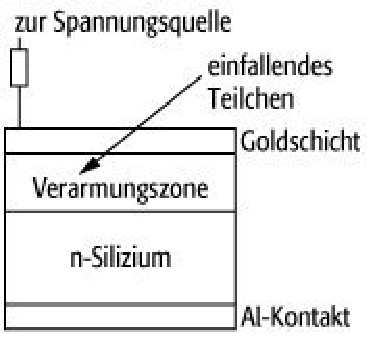
\includegraphics{Oberflaechensperrschichtzaehler.pdf}
\caption{Abbildung \(1\): Oberflächensperrschichtzähler Quelle: \([5]\)}
\end{figure}

Wird eine äußere Spannung angelegt, wächst oder schrumpft die
Verarmungszone, bei ausreichender Spannung verschwindet sie. In
letzterem Fall fließt Strom, daher nennt man diese Richtung
\emph{Durchlassrichtung}. Wird ein Strom in \emph{Sperrrichtung}
angelegt, so wird die Verarmungszone dagegen vergrößert. Daher kann kein
Strom fließen.

Dringt ein \(\alpha\)-Teilchen in die Verarmungszone ein, entstehen
Elektronen-Loch-Paare, während das \(\alpha\)-Teilchen gebremst wird.
Die Elektronen und Löcher werden durch eine anliegende Spannung getrennt
und sammeln sich an den Enden des jeweiligen Halbleiters. Durch einen
empfindlichen Vorverstärker wird ein Spannungsimpuls erzeugt, der von
der Energie des Teilchen abhängt. Um die Verarmungszone und damit das
Detektionsvolumen zu maximieren, wird eine Spannung in Sperrrichtung
angelegt.

Der \(\mathrm{Si}\)-Oberflächen-Sperrschichtzähler besteht aus einen
relativ dicken \(n\)-dotierten Schicht und einer dünnen \(p\)-dotierten
Schicht. Eine sehr dünne Goldschicht sorgt für ein schnelles und
verlustarmes Eindringen der \(\alpha\)-Teilchen. Der schematische Aufbau
eines Oberflächensperrschichtzählers ist in Abbildung \(1\) dargestellt.

Silizium-Halbleiterdetektoren eignet sich aufgrund ihrer Bandlücke von
\(1.11\mathrm{\,eV}\) sehr gut für \(\alpha\)-Strahlung.
Germanium-Halbleiterdetektoren sind prinzipiell ebenfalls geeignet,
müssen allerdings auf ca. \(70\,\mathrm K\) abgekühlt werden. Bei
Raumtemperatur reicht die thermische Energie aus, um die Bandlücke von
\(0.7\mathrm{\,eV}\) zu überwinden. \([6]\)

\hypertarget{durchfuxfchrung}{%
\section{Durchführung}\label{durchfuxfchrung}}

\hypertarget{versuchsaufbau}{%
\subsection{Versuchsaufbau}\label{versuchsaufbau}}

Eine \(^{241}\mathrm{Am}\)-\(\alpha\)-Strahlungsquelle und ein
Silizium-Oberflächensperrschichtzähler sind in einer geschlossenen
Kammer aufgebaut. Zudem gibt es ein Gerüst, in dem sich drei
verschiedene Folien befinden, die zwischen Quelle und Detektor geschoben
werden können. Durch eine Vakuumpumpe kann der Luftdruck in der Kammer
verringert werden.

Der Abstand zwischen Strahlungsquelle und Detektor kann variiert werden,
wobei ein relativer Abstand \(R\) in Millimetern einstellbar ist.

Das Signal des Detektors wird elektronisch verstärkt. Das verstärkte
Zeitsignal wird an einen digitalen Zähler angeschlossen, das verstärkte
Energiesignal kann entweder an ein Oszilloskop oder an einen
Vielkanaldetektor (VKA) angeschlossen werden.

\hypertarget{eichung}{%
\subsection{Eichung}\label{eichung}}

Zunächst wurde das Signal des VKA geeicht. Dazu wurde die Luft aus der
Kammer abgepumpt, bis ein minimaler Druck von ca.
\(1.2\cdot10^{-2}\mathrm{\,mbar}\) erreicht wurde. Dann wurde eine
Messung bei \(R=(0\pm0.5)\mathrm{\,mm}\) mit dem VKA aufgenommen und mit
\texttt{hdtv} \([4]\) ausgewertet.

Hierbei wurde davon ausgegangen, dass der Kanal \(0\) dem
Energienullpunkt entspricht. Weiter wurde angenommen, dass der so
gemessene Peak bei der Energie der \(\alpha\)-Strahlung von
\(5486\mathrm{\,keV}\) liegt, dies war bei Kanal \(10450.4\) der Fall.
Damit wurde \texttt{hdtv} kalibriert.

\hypertarget{energiestraggling}{%
\subsection{Energiestraggling}\label{energiestraggling}}

Um das Energiestraggling zu untersuchen, wurden bei einem eingestellten
relativen Abstand \(R=(18\pm 0.5)\mathrm{\,mm}\) die Energiespektren bei
verschiedenen Drücken \(p_i\) zwischen \(0\mathrm{\,mbar}\) und
\(1013.25\mathrm{\,mbar}=1\mathrm{\,atm}\) aufgenommen. Es wurden \(10\)
Messungen mit einer Dauer von jeweils \(\Delta t=30\mathrm{\,s}\)
getätigt. Diese Messungen wurden sogleich mit \texttt{hdtv} \([4]\)
ausgewertet.

\hypertarget{reichweite-in-luft}{%
\subsection{Reichweite in Luft}\label{reichweite-in-luft}}

Daraufhin wurde die Reichweite der \(\alpha\)-Teilchen gemessen. Dazu
wurden \(4\) verschiedene relative Abstände \(R_i\) eingestellt und je
\(R_i\) Messungen für \(10\) verschiedene Drücke \(p_{i,j}\)
aufgenommen. Hierbei sollten die \(R_i\) größer als die mittlere
Reichweite \(\bar R\) der \(\alpha\)-Teilchen in Luft bei
\(1\mathrm{\,atm}\) sein.

Dabei wurden mittels des digitalen Zählers die Anzahl Detektionen
\(n_i\) sowie die Dauern der Messungen \(\Delta t_i\) aufgezeichnet,
woraus die Zählraten ermittelt werden können. Weiterhin wurden die
Impulshöhen mithilfe des Oszilloskops gemessen.

Die Messungsdauern für die Detektionen unterscheiden sich voneinander,
da versucht wurde, in den meisten Fällen wenigstens \(4500\) Ereignisse
zu messen. Dies soll den statistischen Fehler gering halten. Für die
Messungen mit maximalem Druck wurde dieses Ziel nicht erreicht, hier
wurden maximal \(2\mathrm{\,min}\) lang gemessen.

\hypertarget{metallfolien}{%
\subsection{Metallfolien}\label{metallfolien}}

Zuletzt wurden Folien aus Metall zwischen Strahlungsquelle und Detektor
geschoben. Eine der Folien bestand aus Aluminium, die andere aus Gold.

Die Messungen erfolgten analog zu den Messungen der Reichweite in Luft
(REF), allerdings nur für einen relativen Abstand je Folie. Im Falle von
Aluminium war der relative Abstand \(R_\mathrm{Al}=4\mathrm{\,mm}\), im
Falle von Gold \(R_\mathrm{Au}=8\mathrm{\,mm}\).

\hypertarget{literatur}{%
\section{Literatur}\label{literatur}}

\begin{enumerate}
\def\labelenumi{\arabic{enumi}.}
\tightlist
\item
  K. Bethge, Kernphysik: Eine Einführung, 3. aktualisierte und
  erweiterte Auflage, Springer-Verlag, 2008
\item
  Prior und Rollefson, ``Anomalous energy straggling of alpha
  particles'', American Journal of Physics, Mai 1982,
  \href{https://doi.org/10.1119/1.12834}{DOI 10.1119/1.12834}
\item
  „Chart of Nuclides,`` National Nuclear Data Center,
  \url{https://www.nndc.bnl.gov/nudat3}, \(^{241}_{\ \ 95}\mathrm{Am}\),
  Abruf am 28.01.2024
\item
  Software \href{https://pypi.org/project/hdtv}{\texttt{hdtv}},
  Kurzanleitung unter
  \url{https://www.ikp.uni-koeln.de/fileadmin/data/praktikum/hdtv.pdf},
  Abruf am 28.01.2024
\item
  Lexikon der Physik, Spektrum Verlag,
  \url{https://www.spektrum.de/lexikon/physik/oberflaechensperrschichtzaehler/10568},
  29.01.2024
\item
  G. Knoll, ``Radiation Detection and Measurement'', Wiley, 2010, ISBN:
  9780470131480
\item
  W. Demtröder, ``Experimentalphysik 4: Kern-, Teilchen- und
  Astrophysik'', Springer Spektrum, 2017, ISBN: 9783662528839, DOI:
  \href{https://doi.org/10.1007/978-3-662-52884-6}{10.1007/978-3-662-52884-6}
\end{enumerate}

\end{document}
